\problemname{Strik og Drik}
\section*{Problem Description}
You have been to a “Strik og Drik” event and drank too many gin-hass’. This has resulted in a lot of progress on your project “Blanket for snuggles”, but you have a suspicion that you made some errors along the way. You are fairly new to the knitting world, you only know a couple of knitting patterns, those being:
\begin{itemize}
    \item Stockinette
    \item Lace
    \item Rib
\end{itemize}
In your knitting recipe, you can see that a part of the blanket could look something like this: 
\begin{figure}[h]
    \centering
    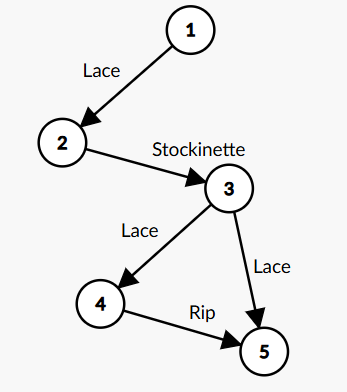
\includegraphics[width=0.2\linewidth]{sample_input.png}
    \caption{A section of your blanket}
    \label{fig:sample_input_4}
\end{figure}\\\\
As the gin-hass' begins to subside, you realised that you accidentally zoned out and knitted your entire blanket. However, you realise that your project is full of mistakes. You have rows where you knitted the wrong patterns, and you have rows where you clearly did follow any distinct pattern. To fix your mistakes you must unravel back to the last correct stitch, so you can restart your blanket.\\\\
Luckily, your blanket closely resembles a directed acyclic graph where:
\begin{itemize}
    \item Each stitch is represented as a node
    \item Each knitting pattern between stitches is a directed edge
    \item Some knitting patterns are mistakes (“DrunkKnitting”)
\end{itemize}
As it really sucks to unravel your entire project, your job is to find the shortest unraveling route from your current stitch back again to the last stitch you remember. To help you achieve this goal, you follow your knitting recipe which states:
\begin{itemize}
    \item Your unraveling route must contain interchanging patterns.
    \item You must end your route when you reach the target pattern ($tp$)
    \item No pattern can be “DrunkKnitting”
\end{itemize}
\section*{Input}
The first line describes the target pattern $tp$.\\
The second line contains two non-negative integers $n$ (number of stitches $2\leq n\leq 100000$) and $m$ (number of edges $1 \leq m \leq (n(n-1)/2)$).\\
The next $m$  lines describe the blanket: \\
$a$   $b$  $pattern$ - describing an edge from stitch $a$ to $b$ with $pattern$ (where $0\leq a < n$ and $a < b <= n$). \\
Patterns are guaranteed to be one of the following ("Stockinette", "Lace", "Rib", "DrunkKnitting").
\section*{Output}
If a valid shortest unraveling route from 1 to $tp$ exists: \\
Print the sequence of patterns used in the route separated by dashes("-").
If no valid path exists, output “Unravel it all :c”